% siminos/atlas/intro.tex  pdflatex atlas
% $Author$ $Date$

\begin{quotation}
The ``lead paragraph'' is encapsulated with the \LaTeX\
\verb+quotation+ environment and is formatted as a single paragraph before the first section heading.
(The \verb+quotation+ environment reverts to its usual meaning after the first sectioning command.)
Note that numbered references are allowed in the lead paragraph.
%
The lead paragraph will only be found in an article being prepared for the journal \textit{Chaos}.
\end{quotation}

    \PC{2012-01-03 experiment with
    \ensuremath{\hat{\ssp}}, \ensuremath{\bar{\ssp}} or \ensuremath{\tilde{\ssp}}
    as the \reducedsp\ coordinate.
    }

\section{Introduction}
\label{s:intro}
% former siminos/atlas/intro.tex

    \PublicPrivate{}{
{\bf 2012-03-12 Predrag} A putative outline of the paper is in
\refsect{chap:atlas}, search for {\bf [2012-03-12 Predrag]}.
    }


The understanding of chaotic dynamics in higher-dimensional systems that
has emerged in the last decade offers a promising dynamical framework to
study turbulence. Here, turbulence is viewed as a walk through a forest
of exact solutions of the governing equations, each solution shaping the
local \statesp\ dynamics.

In this approach, dynamics of moderate \Reynolds\ turbulent flows is
visualized in the $\infty$-dimensional \stateDsp\  using \eqv\ solutions
of the \NSe\ to define dynamically invariant, intrinsic, and
representation independent coordinate frames.
These results inform a new way of thinking about the role {\recurrStr s}
play in shaping turbulence:
The observed {\cohStr s} are the physical images of the flow's
least unstable invariant solutions, with
turbulent dynamics arising from a sequence of transitions between
these states, and
the intrinsic low-dimensionality of turbulence resulting from the low
number of unstable eigendirections for each state.
The unstable \po s are of particular
importance, as they provide the skeleton underpinning the
turbulent dynamics\rf{DasBuch}: the geometry of the \statesp\ flow
near onset of turbulence is shaped by the chaotic saddle, a set of
unstable solutions and their heteroclinic connections.
The long-term goals of this research program are to develop this vision
into quantitative,  predictive description of moderate-{\Reynolds}
turbulence, and to use this description to control flows and explain their statistics.

    \PublicPrivate{}{
In contrast to \pCf, pipe flow has a non-zero mean velocity and cannot
sustain \eqva\ and \po s, so all
unstable invariant solutions are relative, stream-wise traveling
solutions.
    }

Importance of a given invariant solution is made precise by periodic
orbit theory which assigns a deterministic weight with which the solution
contributes to any dynamical average over chaotic component of the flow
\rf{DasBuch}. Consideration of continuous symmetries extends this
theory to sums over \emph{relative} periodic orbits\rf{Cvi07},
time-dependent solutions which recur periodically in co-moving frames
translating and/or rotating along the pipe axis with given stream-wise
and azimuthal velocities, different velocities for each solution.

%%%%%%%%%%%%%%%%%%%%%%%%%%%%%%%%%%%%%%%%%%%%%%%%%
% 2011-10-23 Predrag: replace this Ashley' simulation
%            continuous.tex overheads, and ChaosBook
% TEMPORARY: from siminos/rpo_ks/arxiv-v2/figs, \refref{cont:SCD07})
%
\begin{figure}
\centering
(a)%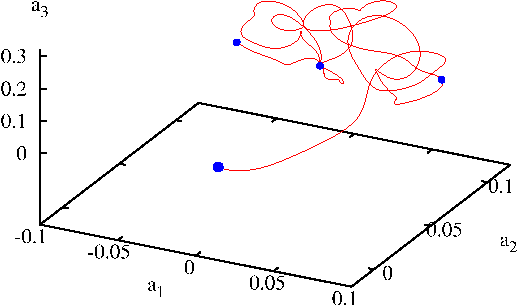
\includegraphics[width=0.45\textwidth,clip=true]{2841GO3a}
~~(b)%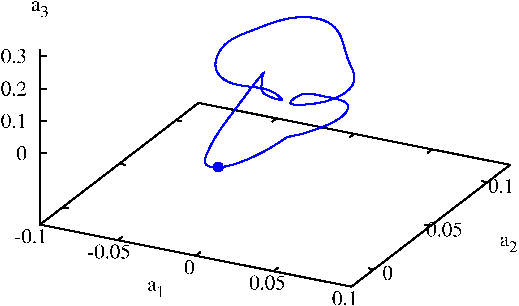
\includegraphics[width=0.45\textwidth,clip=true]{2841GO3b}
  \caption{\label{f:MeanVelocityFrame}
Symmetry reduction $\pS \to \pSRed$ replaces each
(a)
full \statesp\ trajectory $\ssp(\zeit)$ by
(b)
a simpler \reducedsp\ trajectory $\sspRed(\zeit)$, with continuous group
induced drifts quotiented out. Here this is illustrated by the \rpo\
$\RPO{36.92}$ (see \reffig{fig:M1Orb})
(a) %(red)
traced in the full {\statesp} for two $\period{}=36.92$ periods, in the
frame moving with the constant mean axial flow speed $U$ defined in
\refeq{NavStokesDev};
(b) %(blue)
restricted to the symmetry-\reducedsp. Both are projected onto the
$3$\dmn\ frame \refeq{FrenetFrame1}. In the full \statesp\ a \rpo\ traces
out quasi-periodically a highly contorted 2-torus; in the \reducedsp\ it
closes a \po\ in one period $\period{}$.
            }
\end{figure}
%%%%%%%%%%%%%%%%%%%%%%%%%%%%%%%%%%%%%%%%%%%%%%%%%%

In a co-moving frame, moving with the mean phase velocity of a given
solution, a \rpo\ reduces to a \po.
However, as each solution travels with its own mean downstream velocity,
there is no single co-moving frame that can simultaneously reduce
\emph{all} traveling solutions.
    \PC{disparage co-moving frames: they are misleading for \rpo s, as they
    misrepresent time segments for which a \po\ might be glued to
    barely unstable \eqv. A co-moving frame rotates with the constant
    mean
    $\timeAver{\velRel}= \shift_p/\period{p}
    \,.
    $ We \emph{emphatically} do not work in
    co-moving frames.}
    \PC{unhappy about ``moving frames'': misleading, as slice is
     \emph{emphatically} stationary. ''Covariant frames'' move, but we
     do not know how to use them
     }

This problem is here resolved by the
{\mslices}\rf{rowley_reconstruction_2000,BeTh04,SiCvi10,FrCv11}, in
which the group orbit of any full-flow structure is represented by a
single point (see \reffig{fig:BeThTraj}), the group orbit's intersection
with a fixed hypersurface, or the \emph{`\slice'}, analogous to the way a
\PoincSec\ reduces a continuous time orbit to a sequence of points. It
should be noted, however, that a \slice\ is \emph{not} a \PoincSec. A
\slice\ fixes only the group parameters: a continuous time full space
orbit is reduced to a continuous time orbit in the symmetry-\reducedsp,
as in \reffig{f:MeanVelocityFrame}.

Our goals here are two-fold.
(i) We explain what symmetry reduction is, and how with it the geometry
of \statesp\ dynamics is revealed for pipe flow, and
(2) we demonstrate that this new tool enables us to commence a systematic
exploration of the hierarchy of dynamically important invariant solutions
of the pipe flow, starting with two new \rpo s reported here. $3D$
spatial visualization of instantaneous velocity fields,
such as \reffig{fig:N2states}, helps elucidate
the physical processes underlying the formation of unstable coherent
structures. Running concurrently, the $\infty$-dimensional \stateDsp\
representation\rf{GHCW07}, such as \reffig{f:MeanVelocityFrame},
enables us to track the unstable manifolds of invariant
solutions, the heteroclinic connections between them\rf{GHCV08}, and
{provides us with} new insights into the nonlinear \statesp\ geometry and
dynamics of moderate \Reynolds\ wall-bounded flows. Starting in
neighbourhoods of the known \reqva\
 as initial conditions and then searching for
close {recurrences}\rf{pchaot,CviGib10} in the \reducedsp\ yields
educated guesses for locations of \rpo s.

We review  ??? flows, their visualization,
and their symmetries in \refsect{s:review}, where
invariant solutions are classified by their symmetries in
\refappe{appe:DiscSymmPipe}.
The {\mslices}  is described in \refsect{s:slice},
and the computation of invariant solutions and their stability
eigenvalues and eigenvectors in \refsects{s:algorithm}{s:eqbSols}. The
main advances reported in this paper are the symmetry \reducedsp\
visualization and exploration of the moderate-\Reynolds\ turbulent pipe
flow, and determination of new \rpo s\ and their unstable manifolds,
(\refsect{s:rpos}). Outstanding challenges are discussed in
\refsect{s:concl}.
